\chapter{Ziel des Versuchs, Theoretische Grundlagen}
\section{Massenspektrometrie}
Die Massenspektrometrie ist ein typisches Verfahren zur Massenbestimmung von Atomen und Molekülen. Voraussetzung für die Massenspektrometrie ist, das die zu untersuchenden Stoffe (Analyten) mit den verfügbaren Geräten verdampfbar und ionisierbar sind. Um die Verdampfbarkeit und ein gutes Signal zu gewährleisten, wird typischerweise ein sehr geringer Druck benötigt. Die Ionen werden im Massenspektrometer anhand ihres Massenladungsverhältnis $\frac{m}{q}$ sortiert, wobei Moleküle auch fragmentiert werden können. Um die Atome und Moleküle eindeutig zuordnen zu können, ist es nötig eine möglichst große Anzahl an Atom und Molekülmassen zu kennen. Anhand der verschiedenen gemessenen Ionen können dann den gemessenen Massen bestimmte Stoffe zugeordnet werden. 
\subsection{Quadrupolmassenspektrometer}
\label{chapter:QMS}
\begin{figure}
    \centering
    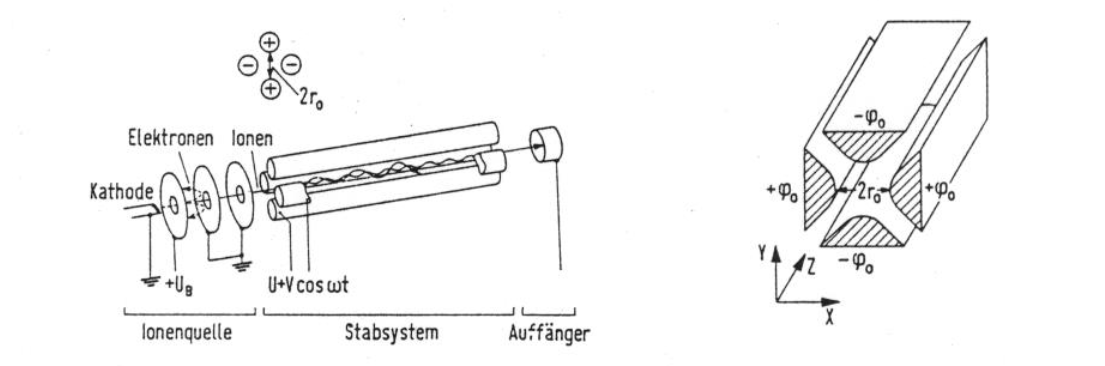
\includegraphics[width=110mm,scale=0.5]{Massenspektrometer/include/quadrupolms.png}
    \caption{Aufbau eines Quadrupolmassenspektrometer \cite{VorbereitungsMappe}}
    \label{fig:quadrupolms}
\end{figure}
In diesem Versuch wird ein Quadrupolmassenspektrometer verwendet. Es ist in Abbildung \ref{fig:quadrupolms} schematisch aufgezeichnet. 

Im QMS werden die Ionen zuerst entlang eines statischen elektrischen Feldes geführt, und fliegen dann parallel zu den 4 Stäben des Stabsystems ein. Zwischen den gegenüberliegenden Stäben ist ein elektrisches Potential mit konstantem Anteil $U$ und oszillierendem Anteil $V\cdot\cos{\omega t}$ angelegt \cite{QMS}. Dies führt dazu das die Bewegungsgleichung der Ionen innerhalb des Potentials der Mathieuschen Differentialgleichung folgt. Die Lösungen dieser Differentialgleichung, die Mathieu-Funktionen, konvergieren für fast alle Parametermöglichkeiten gegen 0 oder unendlich \cite{MathieuscheDiff}. Eine stabile endliche Lösung ergibt sich nur für ein bestimmtes $\frac{m}{q}$ Verhältnis, welches abhängig von den Spannungen $U,V$ und der Frequenz $\omega$ ist. Ionen die ein abweichendes $\frac{m}{q}$-Verhältnis haben, werden noch innerhalb des Stabsystems ausgeworfen und erreichen nicht den Auffänger. Dennoch entsteht hier ein gewisser $\frac{m}{q}$-Akzeptanzbereich, der z.B. durch eine Verlängerung des Stabsystems minimiert werden kann. Über geschickte Einstellung von $U,V, \omega$ kann nun nach bestimmten $\frac{m}{q}$ Verhältnissen gefiltert werden. 
\subsection{Ionenerzeugung}
Damit der Analyt im Stabsystem gefiltert werden kann, muss er ionisierbar sein. Dies kann auf verschiedene Wege stattfinden: 
\subsubsection{Stoßionisation}
Ein Teilchen mit genügend Energie kann bei einem Stoß ein Atom oder Molekül ionisieren. Stoßpartner sind typischerweise Elektronen, Ionen, Photonen oder sogar neutrale Atome. Die nötige Energie kann je nach Teilchen z.B. durch Beschleunigung in einem äußeren elektrischen Feld, oder hohe Temperaturen erreicht werden\cite{Stoßion}. Diese Ionisationsart ist in unserem Experiment dominant. Der hierdurch entstehende Ionisierungsstrom ist druckabhängig und lässt sich somit auch zur Druckbestimmung ausnutzen. 
Der Ionenstrom ist gegeben durch:
$$I = N\cdot Q \cdot l \cdot p \cdot i$$
Wobei $N\cdot Q$ die differentielle Ionisierung, l die Länge des Ionisationsraums, p der Druck und i der Elektronenstrom ist, welcher die Stoßpartner liefert\cite{VorbereitungsMappe}.
\subsubsection{Feldionisation}
In einem starken elektrischen Feld können Elektronen aus ihrer Bindung gelöst werden.
\subsubsection{Autoionisation}
Ein stark angeregtes Atom kann sich spontan selbst ionisieren. 
\subsection{Massenauflösung}
\label{chapter:MSMassenauflösung}
Es gibt eine Vielzahl von möglichen Definitionen der Auflösung eines Massenspektrometers. Im Rahmen dieses Experiments benutzen wir das Auflösungsvermögen $R$ als charakteristische Größe. Diese ist als das Verhältnis einer Masse zur Linienbreite der aufgelösten Masse. $$R = \frac{m}{\Delta m}$$. Auch hier gibt es wieder verschiedene Definitionen von $\Delta m$. Wir wählen hierbei $\Delta m$ als das FWHM eines Peaks.